\newcommand{\ymax}{y_{\mathrm{max}}}
\newcommand{\ymin}{y_{\mathrm{min}}}
\newcommand{\LBMR}{\mathbf{Lbmr}}%%{\Logof{\K_{\GWCM}}}
\newcommand{\height}[1]{\mathrm{h}(#1)}
\newcommand{\clust}[1]{[#1]_\sim}

\section{Bi-relational Kripke Semantics}
\label{sec:bimodels}

% This section presents an alternative connection between the previously
% introduced semantics and another well-known bi-relational semantics.
% This connection has also been considered in~\cite{BP2007,FGMR2024},
% but our approach is simpler and it does not require knowledge of
% universal algebras or descriptive set theory.  In this sense, our
% proposal is very easy to understand.


A \emph{$\GWM$-bimodel} is a structure $\K=\stru{X,\leq,S,V}$ where
$X$ (the set of worlds) is a nonempty finite set, $\leq$ is a partial
order relation, $S\subseteq X \times X$, $V$ (the evaluation function)
is a map from $X$ to $2^\PV$ which is persistent ($x \leq y$ implies
$V(x)\subseteq V(y)$).  We require that $\leq$ satisfies the following
connectedness property:
\begin{itemize}
\item  if $x \leq y$ and $x \leq z$, then $y\leq z$ or $z\leq y$.
\end{itemize}
The  following conditions must be met (see Fig.~\ref{fig:F}):

\begin{enumerate}[label=(F\arabic*), ref=(F\arabic*),leftmargin=*]
\item\label{F1} if $x_1\leq x_2$ and $x_1 S y_1$, there exists $y_2$
  such that $x_2 S y_2$ and $y_1\leq y_2$;
  
%\item\label{F2} if $x_1\leq x_2$ and $x_2 S y_2$, there exists $y_1$
%  such that $x_1 S y_1$ and $y_1\leq y_2$;
  
\item\label{F2} if $x_1 S y_1$ and $y_1\leq y_2$, there exists $x_2$
  such that $x_1\leq x_2$ and $x_2 S y_2$;
  
%\item\label{F4} if $x_2 S y_2$ and $y_1\leq y_2$, there exists $x_1$
%  such that $x_1\leq x_2$ and $x_1 S y_1$;

\item\label{F3} if $x_1 S y_1$ and $x_1 S y_2$ and $y_1 \leq y_2$,
  then $y_1=y_2$;
  
\item\label{F4} if $x_1 S y_1$ and $x_2 S y_1$ and $x_1\leq x_2$, then
  $x_1= x_2$.
\end{enumerate}  
%
%  
% ############################################################
\begin{figure}[t]
  \centering
  \begin{minipage}{12em}
    % F1
    % NODES
    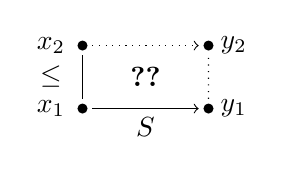
\begin{tikzpicture}[scale=0.8]
      \draw[fill] (0,0) circle (2pt)
      +(0,-0)   node (x1)  {}  % used to label the circle 
      +(-0.5,0) node  {$x_1$}
      ;
      
      \draw[fill] (0,1) circle (2pt)
      +(0,-0)   node (x2)  {}  % used to label the circle 
      +(-0.5,0) node  {$x_2$}
      ;
      
      \draw[fill] (2,0) circle (2pt)
      +(0,-0)   node (y1)  {}  % used to label the circle 
      +(0.4,0) node  {$y_1$}
      ;
      
      
      \draw[fill] (2,1) circle (2pt)
      +(0,-0)   node (y2)  {}  % used to label the circle 
      +(0.4,0) node  {$y_2$}
      ;
      
      
      % ARROWS
      \draw (x1) -- (x2);
      %%\draw[line width=1mm, -{Stealth[length=10mm, open]}] (x1) -- (y1);
      \draw[->] (x1) -- (y1);
      
      \draw[dotted] (y1) -- (y2);
      \draw[->,dotted] (x2) -- (y2);
      
      % NOTES  
      \draw (-0.5,0.5) node{$\leq$}; 
      \draw (1,-0.3) node{$S$}; 
      \draw (1,0.5) node{\ref{F1}}; 
      
      
    \end{tikzpicture}
  \end{minipage}
    % =======================================================
  \begin{minipage}{12em}
    % F2
    % NODES
    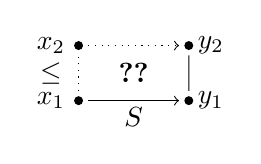
\begin{tikzpicture}[scale=0.7]
      \draw[fill] (0,0) circle (2pt)
      +(0,-0)   node (x1)  {}  % used to label the circle 
      +(-0.5,0) node  {$x_1$}
      ;
      
      \draw[fill] (0,1) circle (2pt)
      +(0,-0)   node (x2)  {}  % used to label the circle 
      +(-0.5,0) node  {$x_2$}
      ;
      
      \draw[fill] (2,0) circle (2pt)
      +(0,-0)   node (y1)  {}  % used to label the circle 
      +(0.4,0) node  {$y_1$}
      ;
      
      
      \draw[fill] (2,1) circle (2pt)
      +(0,-0)   node (y2)  {}  % used to label the circle 
      +(0.4,0) node  {$y_2$}
      ;
      
      
      % ARROWS
      
      \draw[dotted] (x1) -- (x2);
      \draw[->] (x1) -- (y1);
      
      \draw (y1) -- (y2);
      \draw[->,dotted] (x2) -- (y2);
      
      % NOTES  
      \draw (-0.5,0.5) node{$\leq$}; 
      \draw (1,-0.3) node{$S$}; 
      \draw (1,0.5) node{\ref{F2}}; 
      
      
      
    \end{tikzpicture}
  \end{minipage}
  % =======================================================
  \\[2ex]
  \begin{minipage}{12em}
    % F3
    % NODES
    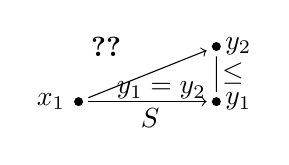
\begin{tikzpicture}[scale=0.7]
      \draw[fill] (0,0) circle (2pt)
      +(0,-0)   node (x1)  {}  % used to label the circle 
      +(-0.5,0) node  {$x_1$}
      ;
      
      
      
      \draw[fill] (2.5,0) circle (2pt)
      +(0,-0)   node (y1)  {}  % used to label the circle 
      +(0.4,0) node  {$y_1$}
      ;
      
      
      \draw[fill] (2.5,1) circle (2pt)
      +(0,-0)   node (y2)  {}  % used to label the circle 
      +(0.4,0) node  {$y_2$}
      ;
      
      
      % ARROWS
      
      \draw[->] (x1) -- (y1);
      \draw[->] (x1) -- (y2);
      \draw (y1) -- (y2);
      
      % NOTES  
      \draw (0.5,1) node{\ref{F3}}; 
      \draw (2.8,0.5) node{$\leq$}; 
      \draw (1.3,-0.3) node{$S$}; 
      \draw (1.5,0.2) node{$y_1=y_2$}; 
      
      
    \end{tikzpicture}
  \end{minipage}
  % =======================================================
  \begin{minipage}{11em}
    % F4
    % NODES
    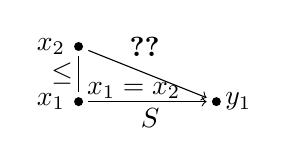
\begin{tikzpicture}[scale=0.7]
      \draw[fill] (0,0) circle (2pt)
      +(0,-0)   node (x1)  {}  % used to label the circle 
      +(-0.5,0) node  {$x_1$}
      ;
      
      \draw[fill] (0,1) circle (2pt)
      +(0,-0)   node (x2)  {}  % used to label the circle 
      +(-0.5,0) node  {$x_2$}
      ;
      
      \draw[fill] (2.5,0) circle (2pt)
      +(0,-0)   node (y1)  {}  % used to label the circle 
      +(0.4,0) node  {$y_1$}
      ;
      
      
      
      % NOTES
      \draw (1.2,1) node{\ref{F4}}; 
      \draw (-0.3,0.5) node{$\leq$}; 
      \draw (1.3,-0.3) node{$S$}; 
      \draw (1,0.2) node{$x_1=x_2$}; 
      
      % ARROWS
      
      \draw[->] (x1) -- (y1);
      \draw[->] (x2) -- (y1);
      \draw (x1) -- (x2);
      
      
    \end{tikzpicture}
  \end{minipage}
  
  
  \caption{Conditions \ref{F1}--\ref{F4}.}
  \label{fig:F}
\end{figure}
%############################################################
%
%
The forcing relation $\forcing$ between worlds of $\K$ and formulas is
defined as follows:
\begin{itemize}
\item $x\nforcing \bot$;
\item $x\forcing p$  iff  $p \in V(x)$, where $p\in\PV$;
\item $x\forcing \a \land \b$ iff $x \forcing \a$ and $x \forcing \b$;
\item $x\forcing \a \lor \b$ iff $x \forcing \a$ or $x \forcing \b$;
\item $x\forcing \a \to \b$ iff for every $x'\in X$ s.t.  $x\leq x'$, if
  $x' \forcing \a$ then $x' \forcing \b$;
\item $x\forcing \Box\a $ iff for every $x',y'\in X$, if $x \leq x'$ and  $x' S y'$  then
  $y'\forcing \a$;
\item $x\forcing \Diam\a $ iff there exists $y\in X$ s.t.~$x S y$ and
  $y \forcing \a$.
\end{itemize}
One can easily prove that forcing is persistent, i.e.: if $x\forcing
\varphi$ and $x\leq x'$, then $x'\forcing\varphi$; in particular,
persistence of $\Diam$-formulas follows from~\ref{F1};
persistence of $\Box$-formulas holds by definition.





% Let $\G$ be a set of formulas.  By $x\forcing\G$ we mean that
% $x\forcing \varphi$, for every $\varphi$ in $\G$.
A formula $\varphi$ is valid in a $\GWM$-bimodel $\K$ iff $x\forcing
\varphi$, for every world $x$ of $\K$.  Let $\LBM$ be
the set of formulas valid in all the $\GWM$-bimodels; we show that
$\LBM$ coincides with $\GWL$.
To this aim, we establish
a correspondence between the class of discrete $\GWM$-models and a particular 
class of $\GWM$-bimodels ensuring that, given any $\M$,  validity in $\M$ simulates
forcing in the corresponding $\K$.


Let $\K=\stru{X,\leq,S,V}$ and let $x$, $y$ be elements of $X$; we set
$x\sim y$ iff $x\leq y$ or $y\leq x$. By the connectedness condition
on $\leq$, $\sim$ is an equivalence relation; we call \emph{clusters}
the $\sim$-equivalence classes.
Let $x\in X$;  by $\clust{x}$ we denote the cluster containing $x$.
If $x$ is not the   $\leq$-minimum element of $\clust{x}$,
there exists a unique world $x'\in\clust{x}$ such that
$x' < x$ and, for
every $y\in \clust{x}$ such that $x'\leq y \leq x$, either $y=x'$ or $y =x$;
we call $x'$ the \emph{immediate $\leq$-predecessor} of $x$. 
Given $x\in X$,
we introduce the following notation:  
\begin{itemize}
\item $\xmin$  is the $\leq$-minimum element in $\clust{x}$;
\item  $\xmax$ is the $\leq$-maximum element in $\clust{x}$;

\item  If $x$ is not the $\leq$-minimum in $\clust{x}$,  $x^-$  is the immediate $\leq$-predecessor
  of $x$.
  
\end{itemize}
Note that, if $x$ is not the  $\leq$-maximum in  $\clust{x}$, then there is $y\in\clust{x}$ such that
$x = y^-$.
The height of a world $x$, denoted by $\height{x}$, is the length 
from $x$ to $\xmax$; formally
\[
  \height{x}\;=\;
  \begin{cases}
0 &\text{if $x$ is the $\leq$-maximum in $\clust{x}$}    
\\
 \height{y} + 1 & \text{if  $x =y^-$}
  \end{cases}
\]
The height of a cluster $\clust{x}$ is the height of $\xmin$.
A model $\K$ is \emph{regular} iff the all the clusters in $\K$ have the same height.


\begin{lemma}\label{lemma:reg}
  Let   $\K=\stru{X,\leq,S,V}$ be a regular model.
\begin{enumerate}[label=(\roman*), ref=(\roman*),leftmargin=*]
\item\label{lemma:reg:1}
  If $ x S y$, then $\height{x}=\height{y}$.

\item\label{lemma:reg:2}
If $x S y$ and  $x^- S y'$ and $y'\in\clust{y}$, then $y'=y^-$.
  
 \end{enumerate}
\end{lemma}

\begin{proof}
    By definition of regular model and conditions \ref{F1}--\ref{F4}.

    **TO DO **
  \end{proof}


By $\LBMR$ we denote the  the set of formulas valid in all regular models.

\begin{lemma}
  $\LBM=\LBMR$
\end{lemma}

\begin{proof}
By definition $\LBM\subseteq \LBMR$. We prove the converse relation, namely  $\LBMR\subseteq \LBM$.

**TO DO **
\end{proof}


\noindent
Let $\K=\stru{X,\leq,S,V}$ be a regular model.
The \emph{height} of $\K$, denoted by $\height{\K}$, is the height of a cluster.
Let  $\height{\K}=k$;  a \emph{ranking} over $\K$ is an order preserving map 
 $\Rn : \{0,\dots, k\} \to (0,1]_\mathrm{Q}$  such that  $\Rnof{k} = 1$.
  The function $\Rn$ is extended to the worlds of $\K$ by setting
 \begin{itemize}
 \item $\Rnof{x} = \Rnof{\height{x}}$, for every $x\in X$.
 \end{itemize}


\noindent
A \emph{ranked $\GWM$-bimodel} is a pair $(\K,\Rn)$, where $\K$ is a regular
$\GWM$-bimodel and $\Rn$ is a ranking over $\K$.
Let $(\K,\Rn)$ be a ranked $\GWM$-bimodel.
By Lemma~\ref{lemma:reg}\ref{lemma:reg:1}, if  $ x S y$, then $\Rnof{x}=\Rnof{y}$.
The rank of a formula $\varphi$ in a cluster $\clust{x}$, denoted by  $\Rnof{\clust{x},\varphi}$
or else by $\Rnof{x,\varphi}$, is defined
as follows:
\[
\Rnof{\clust{x},\varphi} \;=\; \max\left(\,\{\,
  \Rnof{x'}~|~\mbox{$x' \in \clust{x}$ and $x'\forcing\varphi$} 
  \,\}\,\cup\,\{0\}\,\right)
\]
Note that $\Rnof{x,\varphi} \in \Rnof{X}\cup\{0\}$, where $\Rnof{X}$
is the image of $\Rn$.
The following properties immediately follow from the definition of $\Rn$:

 \begin{enumerate}[label=(P\arabic*), ref=(P\arabic*),leftmargin=*]

\item\label{prop:Rn:1}
  $\Rnof{x,\varphi}=0$  iff $\xmax\nforcing \varphi$;
\item\label{prop:Rn:2}
  $\Rnof{x,\varphi}=1$ iff $\xmin\forcing \varphi$; 


\item\label{prop:Rn:3}
  Let $\Rnof{x,\varphi}=r$, where $0 < r < 1$, and let $x_r\in \clust{x}$ be
  such that $\Rnof{x_r} = r$. Then,
  $x_r\forcing \varphi$ and  $(x_r)^-\nforcing \varphi$. 

%\item\label{prop:Rn:4} If $ x S y$,
  

\end{enumerate}

\noindent
Let $x$ and $y$ be two worlds of $\K$; the rank of $S$ w.r.t. the clusters~$\clust{x}$ and $\clust{y}$,
denoted by $\Rnof{S_{\clust{x},\clust{y}}}$   or else by  $\Rnof{S_{x,y}}$,  is defined as follows:
\[
\Rnof{S_{\clust{x},\clust{y}}} \;=\; \max\left(\,\{\,
  \Rnof{x'}~|~\mbox{$x' \in \clust{x}$ and there exists $y'\in\clust{y}$ such that $x'\,S\, y'$} 
  \,\}\,\cup\,\{0\}\,
\right)
\]


% ############################################################## 
%% FIG. RANKED GW-BIMODEL
\begin{figure}[t]
  \centering
    \begin{tikzpicture}[scale=0.8]
      % \begin{tikzpicture}[scale=0.8]
% % OVALS around clusters
       % cluster [y]
       \node[ellipse,draw, fill = gray!10,minimum width = 8em, minimum height = 22ex ] (e) at (-5,4) {};
      
      
      
      % cluster  [x]
       \node[ellipse,draw, fill = gray!10,minimum width = 8em, minimum height = 22ex ] (e) at (0,1.5) {};
      
      
       % cluster [z]
       \node[ellipse,draw, fill = gray!10,minimum width = 8em, minimum height = 22ex ] (e) at (5,4) {};
           
      % WORLDS
      %%% cluster [x]
      % x1
      \draw[fill] (0,0) circle (3pt)
      +(0,-0)   node (x1)  {}  % used to label the circle 
      +(-0.6,0) node  {$x_1$}
      ;
      
      % x08
      \draw[fill] (0,1) circle (3pt)
      +(0,-0)   node (x08)  {}  % used to label the circle 
      +(-0.6,0) node  {$x_{0.8}$}
      ;
      
      % x06
      \draw[fill]  (0,2) circle (3pt)
      +(0,0)   node (x06)  {}  % used to label the circle 
      +(-0.6,0) node  {$x_{0.6}$}
      ;
      
      % x04
      \draw[fill] (0,3) circle (3pt)
      +(0,0)   node (x04)  {}  % used to label the circle 
      +(-0.6,0) node {$x_{0.4}$}  
      ;

      %%% cluster [y]
      % y1
      \draw[fill] (-5,2.5) circle (3pt)
      +(0,-0)   node (y1)  {}  % used to label the circle 
      +(-0.6,0) node  {$y_1$}
      +(0.3,0) node[anchor=west]  {$p$}
      ;

  
      % y08 
      \draw[fill]  (-5,3.5) circle (3pt)
      +(0,0)   node (y08)  {}  % used to label the circle 
      +(-0.6,0) node  {$y_{0.8}$}
      +(0.3,0) node[anchor=west]  {$p$}
      ;

      
      % y06 
      \draw[fill]  (-5,4.5) circle (3pt)
      +(0,0)   node (y06)  {}  % used to label the circle 
      +(-0.6,0) node  {$y_{0.6}$}
      +(0.3,0) node[anchor=west]  {$p$}
      ;
      
      % y04
      \draw[fill] (-5,5.5) circle (3pt)
      +(0,0)   node (y04)  {}  % used to label the circle 
      +(-0.6,0) node  {$y_{0.4}$}
      +(0.3,0) node[anchor=west]  {$p,\,q$}
      ;
      
      %%% cluster [z]
      % z1
      \draw[fill] (5,2.5) circle (3pt)
      +(0,-0)   node (z1)  {}  % used to label the circle 
      +(-0.6,0) node  {$z_1$}
      ;

      % z08 
      \draw[fill]  (5,3.5) circle (3pt)
      +(0,0)   node (z08)  {}  % used to label the circle 
      +(-0.6,0) node  {$z_{0.8}$}
      +(0.3,0) node[anchor=west]  {$q$}
      ;

      
      % z06 
      \draw[fill]  (5,4.5) circle (3pt)
      +(0,0)   node (z06)  {}  % used to label the circle 
      +(-0.6,0) node  {$z_{0.6}$}
      +(0.3,0) node[anchor=west]  {$p,\,q$}
      ;
      
      % z04
      \draw[fill] (5,5.5) circle (3pt)
      +(0,0)   node (z04)  {}  % used to label the circle 
      +(-0.6,0) node  {$z_{0.4}$}
      +(0.3,0) node[anchor=west]  {$p,\,q$}
      ;
            
      % ARROWS
      % <=
      \draw  (x1) -- (x08);
      \draw  (x08) -- (x06);
       \draw  (x06) -- (x04);
      
    \draw  (y1) -- (y08);
      \draw  (y08) -- (y06);
       \draw  (y06) -- (y04);


      \draw  (z1) -- (z08);
      \draw  (z08) -- (z06);
       \draw  (z06) -- (z04);
      

       % S
        \draw[->]  (x08) -- (y08);
        \draw[->]  (x06) -- (y06);
        \draw[->]  (x04) -- (y04);
      
      
        \draw[->]  (x06) -- (z06);
        \draw[->]  (x04) -- (z04);

 %\end{tikzpicture}


%%% Local Variables: 
%%% mode: latex
%%% TeX-master: "goedelModalLogicWitnessNonCrisp"
%%% End: 

          \end{tikzpicture}
\[
    \begin{array}{l}
      \Rnof{0}=0.4,\;\Rnof{1}=0.6,\; \Rnof{2}=0.8,\; \Rnof{3}=1
      \\[0.5ex]
      \Rnof{x_r}=   \Rnof{y_r}=   \Rnof{z_r}= r\qquad
      \Rnof{S_{x_1,y_1}} = 0.8  \qquad  \Rnof{S_{x_1,z_1}} = 0.6 
 \\[0.5ex]
      \Rnof{y_1,p}=1,\quad \Rnof{y_1,q}=0.4,\quad \Rnof{z_1,p}=0.6,\quad \Rnof{z_1,q}=0.8,\quad
      \Rnof{x_1,p}=\Rnof{x_1,q}=0
 \\[1ex]
      \Rnof{y_1,p\land q} =0.4,\quad   \Rnof{y_1,p\lor q} =1,\quad  \Rnof{y_1,p\to q} =0.4\quad \Rnof{y_1,q\to q} = 1,
\\[.5ex]
      \Rnof{y_1,\Box q} =1,\quad \Rnof{y_1,\Diam q} =0
 \\[1ex]
      \Rnof{x_1,\Box p} =1,\quad \Rnof{x_1,\Box q} =0.4,\quad
  \Rnof{x_1,\Diam p} =0.8,\quad \Rnof{x_1,\Diam q} = 0.6
    \end{array}
\]
  \caption{A ranked $\GWM$-bimodel $(\K,\Rn)$ (see Ex.~\ref{ex:rankedBiModel}).}
  \label{fig:rankedBiModel}
\end{figure}
% % ############################################################## 




 \begin{example}\label{ex:rankedBiModel}
   Let us consider the   $\GWM$-bimodel $\K=\stru{X,\leq,S,V}$
   displayed in Fig.~\ref{fig:rankedBiModel}.
The worlds of $\K$ have the form $w_r$, where $w\in\{x,y,z\}$ and  $r\in\{0.4,\,0.6,\,0.8,\,1\}$.
The relation $\leq$ is
  represented by the straight lines ($w\leq w'$ iff $w$ is below or
  equal to $w'$), the relation $S$ is depicted by the arrows.
 The   propositional variables in $V(w_r)$ are displayed to the right of
  $w_r$. 
Formally;
\[
   \begin{array}{l}
%X\;=\;\{\,w_r~|~\text{$w\in\{x,y,z\}$ and  $r\in\{0.4,\,0.6,\,0.8,\,1\}$}   \,\}     
%\qquad
\leq\;=\;\{\,(w_r,w'_{r'})~|~\text{$w=w'$ and $r\geq r'$} \,\}
 \qquad %    \\[1ex]
     S\;=\;\{\, (x_r,y_r)~|~r\leq 0.8 \,\}\;\cup\; \{\, (x_r,z_r)~|~r\leq 0.6 \,\}
     \\[1ex]
     V(w)\;=\;
     \begin{cases}
\{p\}   & \text{if $w\in\{\,y_1,\,y_{0.8},\,y_{0.6} \,\}$}
\\[1ex]
\{q\}   & \text{if $w= z_{0.8}$}
\\[1ex]
 \{p,\,q\}   & \text{if $w\in\{\,y_{0.4},\,z_{0.6},\,z_{0.4} \,\}$}         
\\[1ex]
 \emptyset   & \text{otherwise}         
     \end{cases}
   \end{array}
\]
There are three clusters $\clust{x_1}$, $\clust{y_1}$ and
  $\clust{z_1}$, enclosed in ovals. 
  The model $\K$ is regular. Since  $\K$  has height 3, a ranking over $\K$ has domain $\{0,1,2,3\}$.
  Let $\Rn$ be the ranking function over $\K$ defined as follows:
  \[
  \Rnof{0} = 0.4, \quad  \Rnof{1} = 0.6, \quad  \Rnof{2} = 0.8, \quad   \Rnof{3} = 1
\]
and let us consider the  ranked $\GWM$-bimodel $(\K,\Rn)$.
In  $(\K,\Rn)$, for every world $w_r$ in $\K$  it holds that $\Rnof{w_r}=r$.
Let $w$ and $w'$ be any two worlds of $\K$; then
\[
 \Rnof{S_{w,w'}} \;=\; 
  \begin{cases}
0.8 &\text{if $w=x_1$ and $w'=y_1$}
\\[0.5ex]
 0.6 &\text{if $w=x_1$ and $w'=z_1$}
\\[0.5ex]
0 & \text{otherwise}
  \end{cases}
\]  
In the figure, we show the
ranking of some formulas.
\EndEx
 \end{example}








\begin{lemma}\label{lemma:Rn}
  Let $\K$ be a regular $\GWM$-bimodel and $\Rn$ a ranking over $\K$.
  \begin{enumerate}[label=(\roman*), ref=(\roman*),leftmargin=*]
  \item\label{lemma:Rn:prop}
    $\Rnof{x,\a\star \b}   = \Rnof{x,\a} \star \Rnof{x,\b}$,   for $\star\in \{\,\land,\,\lor,\,\to\,\}$.
    
  \item\label{lemma:Rn:box}
 $\Rnof{x,\Box\a}\,=\min_{y\in X}\{\,\Rnof{S_{x,y}}\to \Rnof{y,\a} \,\}$.
    
  \item\label{lemma:Rn:diam}
    $\Rnof{x,\Diam\a}\,=\,\max_{y\in X}\{\, \Rnof{S_{x,y}} \land \Rnof{y,\a}\,\}$.
  \end{enumerate}
\end{lemma}
\begin{proof}
  \ref{lemma:Rn:prop}.
  We prove that  $\Rnof{x,\a\land \b} =  \Rnof{x,\a}\land  \Rnof{x,\b}$.
  Let $r=\Rnof{x,\a\land \b}$, $a=\Rnof{x,\a}$ and
  $b=\Rnof{x,\b}$; we show that $r= \min(a,b)$.
  Let us assume that $r=0$.
By~\ref{prop:Rn:1},  $\xmax \nforcing \a\land \b$, hence $\xmax \nforcing
  \a$ or $\xmax\nforcing \b$.  In the former case we get $a=0$, in the
  latter $b=0$, hence  $\min(a,b)=0$.
  Let us assume $r=1$. By~\ref{prop:Rn:2},
  $\xmin \forcing \a\land \b$, hence $\xmin \forcing \a$ and
  $\xmin\forcing \b$.  This implies $a=1$ and $b=1$, hence $\min(a,b)=1$.
  Let us assume $0 < r < 1$ and let  $x_r\in \clust{x}$ be
  such that $\Rnof{x_r} = r$.
By~\ref{prop:Rn:3},   $x_r\forcing \a\land \b$ and $(x_r)^-\nforcing \a\land
  \b$, hence $(x_r)^- \nforcing \a$ or $(x_r)^-\nforcing \b$.  
  Let us assume $(x_r)^- \nforcing \a$. Since $x_r\forcing \a$, we get $a=r$;
  moreover, since $x_r\forcing \b$, it holds that  $b\geq r$.
  This proves $\min(a,b)=r$. Likewise, if $(x_r)^- \nforcing \b$, we get
  $b=r$ and $a\geq r$, hence $\min(a,b)=r$.
  This concludes the proof that  $\Rnof{x,\a\land \b} =  \Rnof{x,\a}\land  \Rnof{x,\b}$.
  
  
  The proof of  $\Rnof{x,\a\lor \b}= \Rnof{x,\a}\lor \Rnof{x,\b}$ is similar.

We prove $\Rnof{x,\a\to \b} =\Rnof{x,\a}\to \Rnof{x,\b}$.
  Let $r=\Rnof{x,\a\to \b}$, $a=\Rnof{x,\a}$ and $b=\Rnof{x,\b}$.
  Let us assume $r=0$. By~\ref{prop:Rn:1},  $\xmax \nforcing \a\to \b$,
  hence $\xmax \forcing \a$ and $\xmax \nforcing \b$.  This implies  $a> 0$ 
  and   $b=0$, hence $a\to b = 0$.  Let us assume $r=1$.
 By~\ref{prop:Rn:2},
  $\xmin \forcing \a\to \b$  hence, for every $x'\in\clust{x}$, if $x'\forcing
  \a$ then $x'\forcing \b$. Accordingly, $a \leq b$, and this implies
  $a\to b = 1 $.  Let us assume $0 < r < 1$ and let  $x_r\in \clust{x}$ such that $\Rnof{x_r}=r$.
   By~\ref{prop:Rn:3},  $x_r\forcing \a\to \b$
  and $(x_r)^-\nforcing \a\to \b$; it follows that $(x_r)^-\forcing
  \a$ and $(x_r)^-\nforcing \b$.  Since $(x_r)^-\forcing \a$, we get
  $a \geq \Rnof{(x_r)^-}>r$.  Note that
  $(x_r)^-\nforcing \b$ and $x_r \forcing \b$, hence $b =r$.  It follows that $ a > b$, and this implies $a\to b
  = b $, namely $a\to b= r$.


%###########################################################################

\smallskip
\noindent
\ref{lemma:Rn:box}.
Let $r=\Rnof{x,\Box \a}$; to prove~\ref{lemma:Rn:box}  we show that:

 \begin{enumerate}[label=(\arabic*), ref=(\arabic*),leftmargin=*]
\item\label{lemma:Rn:box:goal}
  $\min_{y\in X}\{\,\Rnof{S_{x,y}}\to \Rnof{y,\a} \,\}\,=\, r$.
\end{enumerate}

\noindent 
Let us assume $r=0$. By~\ref{prop:Rn:1}, it holds that $\xmax \nforcing  \Box \a$, hence
there exists $y^\star\in X$ such that $\xmax S y^\star$ and $y^\star\nforcing \a$.
By Lemma~\ref{lemma:reg}\ref{lemma:reg:1}, $\height{y^\star}=\height{y}$,
hence  $y^\star=\ymax$, and this implies
$\Rnof{y^\star,\a}=0$.
Since $\Rnof{S_{x,y^\star}} > 0$,
we get  $\Rnof{S_{x,y^\star}}\to \Rnof{y^\star,\a}=0$, and this proves~\ref{lemma:Rn:box:goal}.

Let us assume $r=1$. By~\ref{prop:Rn:2},  $\xmin\forcing \Box \a$.
We show that:


 \begin{enumerate}[label=(\alph*), ref=(\alph*),leftmargin=*]
\item\label{lemma:Rn:box:1}
$\Rnof{S_{x,y}}\to \Rnof{y,\a}=1$, for every $y\in X$.
\end{enumerate}
Let $y\in X$.
If $\Rnof{S_{x,y}}=0$, we immediately get $\Rnof{S_{x,y}}\to \Rnof{y,\a}=1$.
Let us assume that   $\Rnof{S_{x,y}} > 0$ and let $x_1\in \clust{x}$
such that $\Rnof{S_{x,y}}=\Rnof{x_1}$.  There exists
$y_1\in \clust{y}$ such that $ x_1 S y_1$;  by Lemma~\ref{lemma:reg}\ref{lemma:reg:1} $\Rnof{y_1} = \Rnof{x_1}$,
thus  $\Rnof{y_1} = \Rnof{S_{x,y}}$.
Since  $\xmin\forcing \Box \a$ and $\xmin\leq x_1$ and $x_1 S y_1$, we get $y_1\forcing \a$, hence $\Rnof{y,\a}\geq \Rnof{y_1}$.
It follows that  $\Rnof{S_{x,y}}\leq\Rnof{y,\a}$,
hence  $\Rnof{S_{x,y}}\to \Rnof{y,\a}=1$, and
this concludes the  proof of~\ref{lemma:Rn:box:1}.
From~\ref{lemma:Rn:box:1}, point~\ref{lemma:Rn:box:goal} follows.


Let us assume $0 < r < 1$ and let  $x_r\in  \clust{x}$ such that  $\Rnof{x_r}=r$.
By~\ref{prop:Rn:3},    $x_r\forcing \Box \a$  and   $(x_r)^-\nforcing \Box \a$. 
There exists $y$ such that $ (x_r)^- S y$ and  $y\nforcing \a$.
By~\ref{F1}, there exists $y_r\in\clust{y}$  such that
$y \leq y_r$ and $x_r S y_r$: by Lemma~\ref{lemma:reg}\ref{lemma:reg:1},
 $\Rnof{y_r} = r$.
We prove that:
\begin{enumerate}[label=(\alph*), ref=(\alph*),leftmargin=*,start=2]
\item\label{lemma:Rn:box:2}
$\Rnof{S_{x,{y_r}}}\to \Rnof{y_r,\a}= r$.
\end{enumerate}


\noindent
Since
 $x_r\forcing \Box \a$ and  $x_r S y_r$, it holds that $y_r\forcing  \a$.
 We have    $y_r\forcing  \a$ and   $y\nforcing \a$.
By Lemma~\ref{lemma:reg}\ref{lemma:reg:2}   $y=( y_r)^-$, hence
 $\Rnof{y_r,\a} = r$.
 Note that $\Rnof{S_{x,{y_r}}}\geq \Rnof{(x_r)^-}  > r$.
 Since  $\Rnof{S_{x,{y_r}}} > r$ and    $\Rnof{y_r,\a} = r$, we get
  $\Rnof{S_{x,y_r}} \to \Rnof{y_r,\a}= r$, and this proves~\ref{lemma:Rn:box:2}.
To complete the proof of~\ref{lemma:Rn:box:goal}, we show that:
\begin{enumerate}[label=(\alph*), ref=(\alph*),leftmargin=*,start=3]
\item\label{lemma:Rn:box:3}
$\Rnof{S_{x,y}}\to \Rnof{y,\a}\geq r$, for every $y\in X$.
\end{enumerate}

\noindent
Let $y\in X$. If $\Rnof{S_{x,y}}\leq \Rnof{y,\a}$, then
$\Rnof{S_{x,y}}\to \Rnof{y,\a} = 1$, hence~\ref{lemma:Rn:box:3} holds.
Let us assume  $\Rnof{S_{x,y}} >  \Rnof{y,\a}$;
then, $\Rnof{S_{x,y}}\to \Rnof{y,\a} =  \Rnof{y,\a}$.
To prove~\ref{lemma:Rn:box:3}, we show that
$\Rnof{y,\a}\geq r$.
Since   $\Rnof{S_{x,y}} > 0$,
there exists $x_1 \in \clust{x}$ such that
$\Rnof{S_{x,y}} =\Rnof{x_1}$. Let $y_1\in \clust{y}$ such that $x_1 S y_1$.
By Lemma~\ref{lemma:reg}\ref{lemma:reg:1} $\Rnof{y_1} = \Rnof{x_1}$,  hence $\Rnof{y_1} > \Rnof{y,\a}$.
It follows that  $y_1\nforcing\a$, hence $x_1\nforcing \Box\a$. Accordingly,
$\Rnof{x_1}> r$, and this implies $x_1 < x_r$. 
Since $\Rnof{S_{x,y}} =\Rnof{x_1}$, by~\ref{F1}  there exists
 $y_r\in\clust{y}$ such that $x_r S y_r$;  by Lemma~\ref{lemma:reg}\ref{lemma:reg:1}, $\Rnof{y_r} = r$. 
Since $x_r\forcing \Box \a$, we get $y_r\forcing \a$; it follows that
$\Rnof{y,\a} \geq r$, and this concludes the proof of~\ref{lemma:Rn:box:3}.



%###########################################################################

\smallskip
\noindent
\ref{lemma:Rn:diam}.
Let $r=\Rnof{x,\Diam \a}$; to prove~\ref{lemma:Rn:diam}  we show that:

 \begin{enumerate}[label=(\arabic*), ref=(\arabic*),leftmargin=*,start=2]
\item\label{lemma:Rn:diam:goal}
  $\max_{y\in X}\{\,\Rnof{S_{x,y}}\land \Rnof{y,\a} \,\}\,=\, r$.
\end{enumerate}
Let us assume $r=0$. By~\ref{prop:Rn:1}, it holds that $\xmax \nforcing  \Diam \a$.
We show that:
 \begin{enumerate}[label=(\alph*), ref=(\alph*),leftmargin=*,start=4]
\item\label{lemma:Rn:diam:1}
$\Rnof{S_{x,y}}\land \Rnof{y,\a}=0$, for every $y\in X$.
\end{enumerate}
Let $y\in X$. If $\Rnof{S_{x,y}}=0$, we immediately get  $\Rnof{S_{x,y}}\land \Rnof{y,\a}=0$.
Let us assume $\Rnof{S_{x,y}} > 0$. Then, there exists $y^\star \in \clust{y}$ such that
$ \xmax S y^\star$. Since  $\xmax \nforcing  \Diam \a$, we get $y^\star\nforcing \a$.
By Lemma~\ref{lemma:reg}\ref{lemma:reg:1},   $\height{y^\star}=0$; as a consequence,    $y^\star = \ymax$ and $\Rnof{y,\a}=0$.
It follows that  $\Rnof{S_{x,y}}\land \Rnof{y,\a}=0$,
and this concludes the proof of~\ref{lemma:Rn:diam:1}. From~\ref{lemma:Rn:diam:1},
~\ref{lemma:Rn:diam:goal} follows.


Let us assume $r=1$. By~\ref{prop:Rn:2},  $\xmin\forcing \Diam \a$.
There exists $y\in X$ such that  $\xmin S y$ and
$y\forcing \a$.
By Lemma~\ref{lemma:reg}\ref{lemma:reg:1}, $\height{y}=\height{\xmin}$;
thus,  $y$ is the $\leq$-minimum world in $\clust{y}$, hence $\Rnof{y,\a}=1$.
Moreover, since $\xmin$ is the $\leq$-minimum world in $\clust{x}$, we get $\Rnof{S_{x,y}}=1$.
It follows that  $\Rnof{S_{x,y}}\land\Rnof{y,\a} =1$, and this proves~\ref{lemma:Rn:diam:goal}.


Let us assume $0 < r < 1$ and let  $x_r\in  \clust{x}$ such that  $\Rnof{x_r}=r$.
By~\ref{prop:Rn:3},    $x_r\forcing \Diam \a$  and   $(x_r)^-\nforcing \Diam \a$. 
There exists $y_r$ such that  $ x_r S y_r$ and  $y_r\forcing \a$;
by Lemma~\ref{lemma:reg}\ref{lemma:reg:1},
 $\Rnof{y_r}= r$, hence $\Rnof{y_r,\a}\geq r$.
We prove that:

\begin{enumerate}[label=(\alph*), ref=(\alph*),leftmargin=*,start=5]
\item\label{lemma:Rn:diam:2}
$\Rnof{S_{x,{y_r}}}\land \Rnof{y_r,\a}= r$.
\end{enumerate}
Since $x_r S y_r$, it holds that $\Rnof{S_{x,{y_r}}}\geq r$.
If  $\Rnof{S_{x,{y_r}}} = r$, we immediately get $\Rnof{S_{x,{y_r}}}\land \Rnof{y_r,\a}= r$.
  Let us assume   $\Rnof{S_{x,{y_r}}}> r$. By~\ref{F1} there exists $y^\star\in \clust{y_r}$ such
  that $(x_r)^- S y^\star$.
  Since $(x_r)^-\nforcing \Diam\a$, we get  $y^\star\nforcing \a$.
  By Lemma~\ref{lemma:reg}\ref{lemma:reg:2} $y^\star =(y_r)^-$, hence $\Rnof{y_r,\a}=r$.
  To sum up,   $\Rnof{S_{x,{y_r}}}> r$ and $\Rnof{y_r,\a}=r$, hence
  $\Rnof{S_{x,{y_r}}}\land \Rnof{y_r,\a}= r$; this proves~\ref{lemma:Rn:diam:2}.
To conclude the proof of~\ref{lemma:Rn:diam:goal},
we show that
  
 \begin{enumerate}[label=(\alph*), ref=(\alph*),leftmargin=*,start=6]
 \item\label{lemma:Rn:diam:3}
 $\Rnof{S_{x,y}}\land \Rnof{y,\a}\leq  r$, for every $y\in X$.
 \end{enumerate}
 Let $y\in X$. If   $\Rnof{S_{x,y}} \leq r$, we immediately get  
 $\Rnof{S_{x,y}}\land \Rnof{y,\a} \leq r$.
 Let us assume  $\Rnof{S_{x,y}} > r$
 and let $x_r\in \clust{x}$ such that $\Rnof{x_r} = r$.
 Note that  $\Rnof{(x_r)^-}\leq \Rnof{S_{x,y}}$,
 hence  there exists $y^\star\in \clust{y}$ such that  $(x_r)^- S y^\star$.
 By Lemma~\ref{lemma:reg}\ref{lemma:reg:1}  $\Rnof{y^\star}= \Rnof{(x_r)^-}$.
 Since $\Rnof{(x_r)^-} > r$, we have $(x_r)^-\nforcing \Diam \a$,
 hence  $y^\star\nforcing \a$.
 It follows that  $\Rnof{y,\a}< \Rnof{y^\star}$, hence   $\Rnof{y,\a}\leq r$.
 This implies  $\Rnof{S_{x,y}}\land \Rnof{y,\a}\leq  r$,
and this proves~\ref{lemma:Rn:diam:3}.
\end{proof}


  
\noindent
A \emph{correspondence} between a discrete $\GWM$-model $\M=\stru{W,R,e}$ and a ranked
$\GWM$-bimodel $(\K,\Rn)$, where $\K=\stru{X,\leq,S,V}$ is a regular model, is a 1-1 map
$\Phi$ between the worlds of $\M$ and the clusters of $\K$ satisfying
the following conditions:






  \begin{enumerate}[label=(C\arabic*), ref=(C\arabic*),leftmargin=*]

  \item\label{corr:1}
    $R(w_1, w_2)=\Rnof{ S_{\Phi(w_1),\Phi(w_2)}  }$, for every
  $w_1,w_2\in W$;

\item\label{corr:2}
  $e(w,p) =\Rnof{\Phi(w),p}$, for every $w\in W$ and $p\in\PV$.
\end{enumerate}
 



 
%% FIG. MODEL - CORRESPONDENCE
\begin{figure}[t]
  \centering
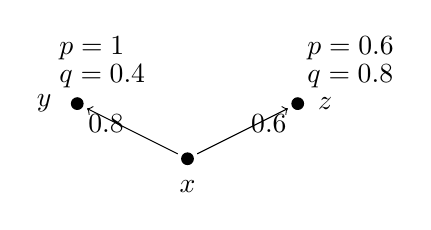
\begin{tikzpicture}[scale=0.7]
  %% Model M = < W,R,e>
  % WORLDS  
      % x
      \draw[fill] (0,0) circle (3pt)
      +(0,0)   node (x)  {}  % used to label the circle 
      +(0,-0.5) node  {$x$}
      ;
      
      % y 
      \draw[fill]  (-2,1) circle (3pt)
      +(0,0)   node (y)  {}  % used to label the circle 
      +(-0.6,0)  node  {$y$}
      +(-0.5,0.5) node[anchor=west]  {$q=0.4$}
      +(-0.5,1) node[anchor=west]  {$p=1$}
      ;
      
      % z
      \draw[fill] (2,1) circle (3pt)
      +(0,0)   node (z)  {}  % used to label the circle 
      +(0.5,0) node{$z$}
      +(0,0.5) node[anchor=west]  {$q = 0.8$}
      +(0,1) node[anchor=west]  {$p=0.6$}
      ;
      
      % ARROWS
      \draw[->] (x) -- (y) node[below right=0.5] {0.8}  ;
      \draw[->] (x) -- (z) node[below left=0.5] {0.6}  ;
    \end{tikzpicture}\begin{tikzpicture}[scale=0.7]
      % \begin{tikzpicture}[scale=0.8]
% % OVALS around clusters
       % cluster [y]
       \node[ellipse,draw, fill = gray!10,minimum width = 8em, minimum height = 22ex ] (e) at (-5,4) {};
      
      
      
      % cluster  [x]
       \node[ellipse,draw, fill = gray!10,minimum width = 8em, minimum height = 22ex ] (e) at (0,1.5) {};
      
      
       % cluster [z]
       \node[ellipse,draw, fill = gray!10,minimum width = 8em, minimum height = 22ex ] (e) at (5,4) {};
           
      % WORLDS
      %%% cluster [x]
      % x1
      \draw[fill] (0,0) circle (3pt)
      +(0,-0)   node (x1)  {}  % used to label the circle 
      +(-0.6,0) node  {$x_1$}
      ;
      
      % x08
      \draw[fill] (0,1) circle (3pt)
      +(0,-0)   node (x08)  {}  % used to label the circle 
      +(-0.6,0) node  {$x_{0.8}$}
      ;
      
      % x06
      \draw[fill]  (0,2) circle (3pt)
      +(0,0)   node (x06)  {}  % used to label the circle 
      +(-0.6,0) node  {$x_{0.6}$}
      ;
      
      % x04
      \draw[fill] (0,3) circle (3pt)
      +(0,0)   node (x04)  {}  % used to label the circle 
      +(-0.6,0) node {$x_{0.4}$}  
      ;

      %%% cluster [y]
      % y1
      \draw[fill] (-5,2.5) circle (3pt)
      +(0,-0)   node (y1)  {}  % used to label the circle 
      +(-0.6,0) node  {$y_1$}
      +(0.3,0) node[anchor=west]  {$p$}
      ;

  
      % y08 
      \draw[fill]  (-5,3.5) circle (3pt)
      +(0,0)   node (y08)  {}  % used to label the circle 
      +(-0.6,0) node  {$y_{0.8}$}
      +(0.3,0) node[anchor=west]  {$p$}
      ;

      
      % y06 
      \draw[fill]  (-5,4.5) circle (3pt)
      +(0,0)   node (y06)  {}  % used to label the circle 
      +(-0.6,0) node  {$y_{0.6}$}
      +(0.3,0) node[anchor=west]  {$p$}
      ;
      
      % y04
      \draw[fill] (-5,5.5) circle (3pt)
      +(0,0)   node (y04)  {}  % used to label the circle 
      +(-0.6,0) node  {$y_{0.4}$}
      +(0.3,0) node[anchor=west]  {$p,\,q$}
      ;
      
      %%% cluster [z]
      % z1
      \draw[fill] (5,2.5) circle (3pt)
      +(0,-0)   node (z1)  {}  % used to label the circle 
      +(-0.6,0) node  {$z_1$}
      ;

      % z08 
      \draw[fill]  (5,3.5) circle (3pt)
      +(0,0)   node (z08)  {}  % used to label the circle 
      +(-0.6,0) node  {$z_{0.8}$}
      +(0.3,0) node[anchor=west]  {$q$}
      ;

      
      % z06 
      \draw[fill]  (5,4.5) circle (3pt)
      +(0,0)   node (z06)  {}  % used to label the circle 
      +(-0.6,0) node  {$z_{0.6}$}
      +(0.3,0) node[anchor=west]  {$p,\,q$}
      ;
      
      % z04
      \draw[fill] (5,5.5) circle (3pt)
      +(0,0)   node (z04)  {}  % used to label the circle 
      +(-0.6,0) node  {$z_{0.4}$}
      +(0.3,0) node[anchor=west]  {$p,\,q$}
      ;
            
      % ARROWS
      % <=
      \draw  (x1) -- (x08);
      \draw  (x08) -- (x06);
       \draw  (x06) -- (x04);
      
    \draw  (y1) -- (y08);
      \draw  (y08) -- (y06);
       \draw  (y06) -- (y04);


      \draw  (z1) -- (z08);
      \draw  (z08) -- (z06);
       \draw  (z06) -- (z04);
      

       % S
        \draw[->]  (x08) -- (y08);
        \draw[->]  (x06) -- (y06);
        \draw[->]  (x04) -- (y04);
      
      
        \draw[->]  (x06) -- (z06);
        \draw[->]  (x04) -- (z04);

 %\end{tikzpicture}


%%% Local Variables: 
%%% mode: latex
%%% TeX-master: "goedelModalLogicWitnessNonCrisp"
%%% End: 

    \end{tikzpicture}
%%%%%%%%%%%%%%%%%%%%%%%%%%%%
 \[
  \begin{array}{l}
    \Phi(x)=\clust{x_1} \qquad \Phi(y)=\clust{y_1}\qquad  \Phi(z)=\clust{z_1}
  \end{array}
 \] 
          \caption{A correspondence $\Phi$ between the model $\M=\stru{W,R,e}$ and the ranked   $\GWM$-bimodel $(\K,\Rn)$
            (see  Ex.~\ref{ex:corr}).}
  \label{fig:modelCorrespondence}
\end{figure}





\begin{example}\label{ex:corr}
In    Fig.~\ref{fig:modelCorrespondence} we show a correspondence $\Phi$
between the discrete model $\M=\stru{W,R,e}$  shown on  the left and 
the ranked $\GWM$-bimodel $(\K,\Rn)$  represented on the right  (see Ex.~\ref{ex:rankedBiModel}).

\[
\Phi(x)=\clust{x_1} \qquad \Phi(y)=\clust{y_1}\qquad  \Phi(z)=\clust{z_1}
 \]
 Note that, for every world $w$ in $\M$ and every   formula $\varphi$,
 it holds that  $e(w,\varphi)=\Rnof{\Phi(w),\varphi}$; this crucial property is proved in next lemma. 
   \EndEx  
 \end{example}



\begin{proposition}\label{prop:Phi}
  Let $\Phi$ be a correspondence between $\M$ and  $(\K,\Rn)$.
  For every formula $\varphi$ and every world $w$ of $\M$,
  $e(w,\varphi) =\Rnof{\Phi(w),\varphi}$.
\end{proposition}



\begin{proof}
Let $w\in W$ and $\varphi$ any formula; we prove  $e(w,\varphi) =\Rnof{\Phi(w),\varphi}$
  by induction on the size of $\varphi$. If $\varphi\in\PV$,
   the assertion immediately follows from~\ref{corr:2}.
   The case  $\varphi =\bot$ is trivial, since  $e(w,\bot)=0$
   and $\Rnof{\Phi(w),\bot}=0$.

   Let $\varphi=\a\star \b$, where $\star\in \{\,\land,\,\lor,\,\to\,\}$. We have:
   \[
     e(w, \a\star \b) \,= \, e(w,\a)\star (w,\b)
     \,\stackrel{(\dag)}{=}\,
     \Rnof{\Phi(w),\a}\star  \Rnof{\Phi(w),\b} 
 \,\stackrel{(\ddag)}{=}\,
     \Rnof{\Phi(w),\a\star \b}
   \]
   where $(\dag)$ follows from the induction hypothesis and $(\ddag)$
   from Lemma~\ref{lemma:Rn}\ref{lemma:Rn:prop}.

Let $\M=\stru{W,R,e}$ and  $\K=\stru{X,\leq,S,V}$.
We have:
\[
  \begin{array}{rcll}
  e(w,\Box \a) & \;=\; & \min_{w'\in W}\{\, R(w,w') \to e(w',\a) \,\}    
&
    \\[.5ex]
 & \;=\; & \min_{w'\in W}\{\, \Rnof{S_{\Phi(w),\Phi(w')} } \to e(w',\a) \,\}    
&\text{\ref{corr:1}}
    \\[.5ex]
               & \;=\; &
   \min_{w'\in W}\{\, \Rnof{S_{\Phi(w),\Phi(w')} } \to \Rnof{\Phi(w'),\a} \,\}
&\text{ind.~hyp.}
\\[.5ex]
 & \;=\; &
   \min\;\underbrace{\{\, \Rnof{S_{\Phi(w),\Phi(w')} } \to \Rnof{\Phi(w'),\a}~|~w'\in W \,\}}_{\Qcal_1}                         
&
%======================================
    \\[5ex]
    \Rnof{\Phi(w),\Box \a}   & \;=\; &
                                       \min_{y\in X}\{\, \Rnof{S_{\Phi(w),y} } \to \Rnof{y,\a} \,\}
&\text{ Lemma~\ref{lemma:Rn}\ref{lemma:Rn:box}}
\\[.5ex]
 & \;=\; &
 \min\;\underbrace{\{\, \Rnof{S_{\Phi(w),y} } \to \Rnof{y,\a}~|~y\in X \,\}}_{\Qcal_2}
    \end{array}
\]
We show that  $\Qcal_1=\Qcal_2$.
Let $q_1\in \Qcal_1$ and let us assume that
$q_1=\Rnof{S_{\Phi(w),\Phi(w')} } \to \Rnof{\Phi(w'),\a}$, where $w'\in W$.  
Let $y\in \Phi(w')$; 
then $\clust{y}=\Phi(w')$ hence:
\[
  \Rnof{S_{\Phi(w),y}}\to  \Rnof{y,\a} \,\in \Qcal_2
  \qquad
  \Rnof{S_{\Phi(w),y}}= \Rnof{S_{\Phi(w),\Phi(w')}}
  \qquad
 \Rnof{y,\a}  = \Rnof{\Phi(w'),\a}  
\]  
This implies  $q_1\in\Qcal_2$. Conversely, let $q_2\in\Qcal_2$
and let us assume that $q_2=  \Rnof{S_{\Phi(w),y}}\to  \Rnof{y,\a}$.
Then, there exists $w'\in W$ such that $\Phi(w') = \clust{y}$, hence:
\[
  \Rnof{S_{\Phi(w),\Phi(w')}}\to  \Rnof{\Phi(w'),\a} \,\in \Qcal_1
  \qquad
\Rnof{S_{\Phi(w),\Phi(w')}} =  \Rnof{S_{\Phi(w),y}}
  \qquad
 \Rnof{\Phi(w'),\a} =  \Rnof{y,\a} 
\]  
Accordingly  $q_2\in\Qcal_1$. Having proved that $\Qcal_1=\Qcal_2$, we conclude
 $e(w,\Box \a)  = \Rnof{\Phi(w),\Box \a}$. 

 The proof of  $e(w,\Diam \a)  = \Rnof{\Phi(w),\Diam \a}$ is similar.
\end{proof}




To show that $\LBMR$ and $\GWL$ coincide, we need the following lemma:

\begin{lemma}\label{lemma:Phi}
\text{}
  \begin{enumerate}[label=(\roman*), ref=(\roman*),leftmargin=*]
  \item\label{lemma:Phi:MtoK} Let $\M$ be a discrete
    $\GWM$-model.  Then, there exists a ranked $\GWM$-bimodel
    $(\K,\Rn)$ and a correspondence $\Phi$ between $\M$ and
    $(\K,\Rn)$.
    
  \item\label{lemma:Phi:KtoM}
    Let  $(\K,\Rn)$ be a  ranked  $\GWM$-bimodel.
    Then, there exists  a  discrete $\GWM$-model  $\M$ and
    a correspondence $\Phi$ between $\M$ and  $(\K,\Rn)$.
  \end{enumerate}
  
\end{lemma}



\begin{proof}
  \ref{lemma:Phi:MtoK}. Let $\M=\stru{W,R,r}$ and let
  $\Qcal = (e(W)\cup R(W) \cup \{1\}) \setminus \{0\}$; since $\M$ is discrete, $\Qcal$ is a
finite subset of $(0,1]_Q$.  The $\GWM$-bimodel $\K=\stru{X,\leq,S,V}$
and the map $\Rn$ are defined as follows:
\[
  \begin{array}{ll}
    X\;=\;\{\, w_r~|~ r\in \Qcal\,\}
&    
\leq \;=\; \{\, (w_r, w'_{r'})~|~\text{$w = w'$ and $r \geq r'$ }  \,\}    
\\[1ex]
    S \;=\; \{\, (w_r, w'_{r'})~|~\text{$r = r'$ and $r \leq R(w,w')$ }  \,\}
&
V \;=\; \{\, (w_r, p)~|~\text{ $r \leq e(w,p)$ }  \,\}
\end{array}
\]
    One can easily  check that $\K$ is a  well-defined regular model.
   For every $w\in W$, the set of  $w_r$ such that $r\in \Qcal$ is a cluster of $\K$.
    Let us assume that $\Qcal$ contains $k+1$ elements  ($k\geq 0$) and let 
    $r_0,r_1, \dots, r_{k}$ be an enumeration of the elements of $\Rcal$ in ascending order
    (thus, $r_k=1$).
   The map $\Rn : \{0,\dots,k\}\to\Qcal$
    such that $\Rnof{k} = r_k$ is a ranking over $\K$.  Note that $\Rnof{w_j}=r_j$.
    The function $\Phi$ mapping the world $w$ of $\M$ to the cluster
    $\clust{w_1}$ settles a correspondence between $\M$ and  $(\K,\Rn)$. 

    \smallskip
    \noindent
   \ref{lemma:Phi:KtoM}
   Let  $\K=\stru{X,\leq,S,V}$.
   The  $\GWM$-model  $\M=\stru{W,R,e}$ is defined as follows:
   \[
     \begin{array}{l}
W\,=\,\{\, \clust{x}~|~x\in W   \,\}
       \qquad
       R(\clust{x},  \clust{x'}) \,=\, \Rnof{S_{x,x'}}
\qquad
e(\clust{x},p)\,=\, \Rnof{\clust{x},p}
     \end{array}
\]
One can easily check that $\M$ is well-defined.  Let $\Phi$ be the map
between the worlds of $\M$ and the clusters of $\K$ such that,
given a    a world $\clust{x}$ of $\M$, $\Phi(\clust{x})=\clust{x}$.
One can easily check that   $\Phi$
   is  a correspondence between $\M$ and  $(\K,\Rn)$. 
 \end{proof}



\begin{figure}[t]
  \centering
  \begin{minipage}{12em}
      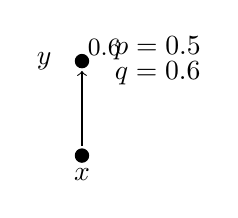
\begin{tikzpicture}[scale=0.8]
        % WORLDS  
        % x
        \draw[fill] (0,0) circle (3pt)
        +(0,-0)   node (x)  {}  % used to label the circle 
        +(0,-0.3) node  {$x$}
        ;
        
        % y 
        \draw[fill]  (0,1.5) circle (3pt)
        +(0,0)   node (y)  {}  % used to label the circle 
        +(-0.6,0)  node  {$y$} 
        +(1.2,0.2) node  {$p=0.5$}
        +(1.2,-0.2) node  {$q=0.6$}
        ;
        
        
        % ARROWS
        \draw[->] (x) -- (y) node[above right=-1.4] {{\small 0.6}} ;
      \end{tikzpicture}
\end{minipage}\begin{minipage}{15em}
      \begin{tikzpicture}[scale=0.8]
%====================================================================
        %% RANKED BI-MODEL
      % % OVALS around clusters
       % cluster [y]
       \node[ellipse,draw, fill = gray!10,minimum width = 6em, minimum height = 16ex ] (e) at (0,1) {};
      
      
      
      % cluster  [x]
       \node[ellipse,draw, fill = gray!10,minimum width = 6em, minimum height = 16ex ] (e) at (4,1) {};
      
      
           
      % WORLDS
      %%% cluster [x]
      % x1
      \draw[fill] (0,0) circle (3pt)
      +(0,-0)   node (x1)  {}  % used to label the circle 
      +(-0.6,0) node  {$x_1$}
      ;
      
      % x06
      \draw[fill] (0,1) circle (3pt)
      +(0,-0)   node (x06)  {}  % used to label the circle 
      +(-0.6,0) node  {$x_{0.6}$}
      ;
      
      % x05
      \draw[fill]  (0,2) circle (3pt)
      +(0,0)   node (x05)  {}  % used to label the circle 
      +(-0.6,0) node  {$x_{0.5}$}
      ;
      

      %%% cluster [y]
      % y1
      \draw[fill] (4,0) circle (3pt)
      +(0,-0)   node (y1)  {}  % used to label the circle 
      +(-0.6,0) node  {$y_1$}
      ;

  
      % y06 
      \draw[fill]  (4,1) circle (3pt)
      +(0,0)   node (y06)  {}  % used to label the circle 
      +(-0.6,-0.2) node  {$y_{0.6}$}
      +(0.1,0) node[anchor=west]  {$q$}
      ;

      
      % y05 
      \draw[fill]  (4,2) circle (3pt)
      +(0,0)   node (y05)  {}  % used to label the circle 
      +(-0.6,-0.2) node  {$y_{0.5}$}
      +(0.1,0) node[anchor=west]  {$p,\,q$}
      ;
      
             
      % ARROWS
      % <=
      \draw  (x1) -- (x06);
      \draw  (x06) -- (x05);
      
    \draw  (y1) -- (y06);
      \draw  (y06) -- (y05);
 
      

       % S
        \draw[->]  (x06) -- (y06);
         \draw[->]  (x05) -- (y05);
      
   \end{tikzpicture}
 \end{minipage}
\\[1ex]
 $\Phi(x) = \clust{x_1}\qquad  \Phi(y) = \clust{y_1}$
   \[\small
    \begin{array}{rclcl}
      e(x,\Box (p\lor q))&=& 1 &=& \Rnof{x,\Box(p\lor q)}
      \\[1ex]
      e(x,\Box p) &=&  0.5&=& \Rnof{x,\Box p)}
      \\[1ex]
      e(x,\Diam q)&=&  0.6 &=& \Rnof{x,\Diam q}
      \\[1ex]
      e(x,\varphi) &=& 0.6  &=& \Rnof{x,\varphi}
    \end{array}
  \]
  
  \caption{A $\GWM$-countermodel for the formula $\varphi=\Box (p\lor q)\to
    (\Box p \lor \Diam q) $ (instance of (Cr)) and the corresponding ranked $\GWM$-bimodel.}
  \label{fig:corrCrispAx}
\end{figure}



 
 \begin{example}
Let us consider the $\GWM$-countermodel $\M$ for the formula $\varphi=\Box (p\lor q)\to (\Box p \lor \Diam q) $ (instance of (Cr)) 
shown in Fig.~\ref{fig:corrCrispAx} on the left.
On the right of the figure, we define the ranked $\GWM$-bimodel $(\K,\Rn)$  corresponding to $\M$ obtained by applying the
procedure described in the proof of  Lemma~\ref{lemma:Phi}\ref{lemma:Phi:MtoK}. 
Since $e(x,\varphi) = 0.6$, it follows that $\Rn{\clust{x_1}}=0.6$. Since $\Rnof{x_1}=1$, it holds that
$x_1\nforcing \varphi$; accordingly, $\K$ is a countermodel for $\varphi$.
 \end{example}



\begin{proposition}\label{prop:equivGWC}
  $\LBMR =\GWL$.
\end{proposition}

\begin{proof}
Let $\varphi\not\in \GWL$. By the completeness theorem, 
there exist a discrete $\GWM$-model $\M=\stru{W,R,e}$ and $w\in W$ such that $e(w,\varphi)<1$.
By Lemma~\ref{lemma:Phi}\ref{lemma:Phi:MtoK} there is a ranked
$\GWM$-bimodel $(\K,\Rn)$ and a correspondence $\Phi$ between $\M$
and $(\K,\Rn)$. By Prop.~\ref{prop:Phi}, $\Rnof{\Phi(w),\varphi} =
e(w,\varphi)$, hence $\Rnof{\Phi(w),\varphi} < 1$.  This implies that there
exists $x\in \Phi(w)$ such that $x\nforcing \varphi$; thus
$\varphi\not\in \LBM$. This proves that $\LBM\subseteq \GWL$.  The
proof of $\GWL\subseteq \LBM$ is similar and relies on
Lemma~\ref{lemma:Phi}\ref{lemma:Phi:KtoM}.
  
\end{proof}


\subsection{On condition \ref{F4}}

  
%############################################################
\begin{figure}[t]
  \centering
  \begin{minipage}{9em}\small\center
% F1 countermodel
% NODES
    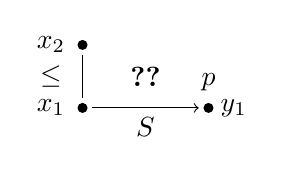
\begin{tikzpicture}[scale=0.8]
 \draw[fill] (0,0) circle (2pt)
   +(0,-0)   node (x1)  {}  % used to label the circle 
  +(-0.5,0) node  {$x_1$}
  ;

 \draw[fill] (0,1) circle (2pt)
   +(0,-0)   node (x2)  {}  % used to label the circle 
  +(-0.5,0) node  {$x_2$}
  ;

\draw[fill] (2,0) circle (2pt)
   +(0,-0)   node (y1)  {}  % used to label the circle 
   +(0.4,0) node  {$y_1$}
    +(0,0.4) node  {$p$}
  ;



% ARROWS
  
\draw (x1) -- (x2);
\draw[->] (x1) -- (y1);
  

% NOTES  
\draw (-0.5,0.5) node{$\leq$}; 
\draw (1,-0.3) node{$S$}; 
  \draw (1,0.5) node{\ref{F1}}; 


\end{tikzpicture}
$\varphi= \Diam p\to \neg\neg\Diam p$
     \end{minipage}
%=======================================================
\begin{minipage}{9em}\small\center
% F2 countermodel
% NODES
    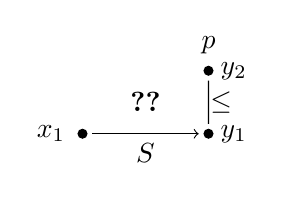
\begin{tikzpicture}[scale=0.8]
 \draw[fill] (0,0) circle (2pt)
   +(0,-0)   node (x1)  {}  % used to label the circle 
  +(-0.5,0) node  {$x_1$}
  ;


\draw[fill] (2,0) circle (2pt)
   +(0,-0)   node (y1)  {}  % used to label the circle 
  +(0.4,0) node  {$y_1$}
  ;


\draw[fill] (2,1) circle (2pt)
   +(0,-0)   node (y2)  {}  % used to label the circle 
   +(0.4,0) node  {$y_2$}
    +(0,0.4) node  {$p$}
  ;


% ARROWS
  

\draw[->] (x1) -- (y1);
  
\draw (y1) -- (y2);


% NOTES
\draw (2.2,0.5) node{$\leq$};
\draw (1,-0.3) node{$S$}; 
  \draw (1,0.5) node{\ref{F2}}; 



\end{tikzpicture}
$\varphi= \Diam\neg\neg  p\to \neg\neg \Diam p$
  \end{minipage}
%=======================================================
     \begin{minipage}{9em}\small\center
% F3 countermodel
% NODES
    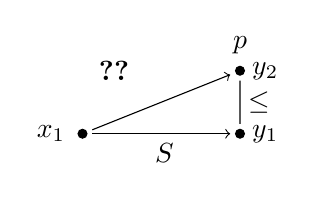
\begin{tikzpicture}[scale=0.8]
 \draw[fill] (0,0) circle (2pt)
   +(0,-0)   node (x1)  {}  % used to label the circle 
  +(-0.5,0) node  {$x_1$}
  ;



\draw[fill] (2.5,0) circle (2pt)
   +(0,-0)   node (y1)  {}  % used to label the circle 
  +(0.4,0) node  {$y_1$}
  ;


\draw[fill] (2.5,1) circle (2pt)
   +(0,-0)   node (y2)  {}  % used to label the circle 
   +(0.4,0) node  {$y_2$}
    +(0,0.4) node  {$p$}
  ;


% ARROWS
  
 \draw[->] (x1) -- (y1);
 \draw[->] (x1) -- (y2);
 \draw (y1) -- (y2);

 % NOTES  
\draw (0.5,1) node{\ref{F3}}; 
\draw (2.8,0.5) node{$\leq$}; 
\draw (1.3,-0.3) node{$S$}; 

       \end{tikzpicture}
$\varphi= \Box \neg\neg p\to \neg\neg \Box p$
     \end{minipage}
  
  \caption{In each model $x_1\nforcing\varphi$, where $\varphi\in\GWL$.}
  \label{fig:Fcountermodels}
\end{figure}
%############################################################



To give a bi-relational Kripke semantics of $\GWL$, we have introduced the
conditions~\ref{F1}-\ref{F4}.  As reported in
Fig.~\ref{fig:Fcountermodels}, if any of the conditions~\ref{F1},
\ref{F2}, and~\ref{F3}  is ruled out, we can build a
countermodel for a formula of $\GWL$. For instance, let us consider
the left-most $\GWCM$-bimodel $\K=\stru{X,\leq,S,V}$, where $x_1 <
x_2$, $x_1 S y_1$, $V(y_1)=\{p\}$; $\K$ does not match
condition~\ref{F1}, moreover $\K$ is a countermodel for the formula
$\varphi= \Diam p\to \neg\neg\Diam p$ of $\GWL$ (indeed,
$x_1\nforcing \varphi$). A similar analysis applies to conditions~\ref{F2} and \ref{F3}.

On the contrary, it seems that it is
not possible to build a countermodel $\K$ for a formula $\varphi$ of
$\GWCL$ violating condition~\ref{F4};
 actually, we conjecture that condition~\ref{F4} is redundant.

 

%%% Local Variables: 
%%% mode: latex
%%% TeX-master: "goedelModalLogicWitnessNonCrisp"
%%% End: 
